%%%%%%%%%%%%%%%%%%%%%%%%%%%%%%%%%%%%%%%%%%%%%%%%%%%%%%%%%%%%%%%%%%%%%%%%%%%%%%%%%%%%%%%%%%%%%%%%%%%%%%%%%%%%%%%%%%%%%%%%%%%%%%%%
% Chapitre 1
\chapter{Chapitre 1 : Intelligence artificielle générative}
%%%% Intro du Chapitre
\phantomsection
\section*{Introduction}
\addcontentsline{toc}{section}{Introduction}
\paragraph{}
En quoi consiste l’IA générative ?
L'intelligence artificielle générative est une catégorie d'IA qui se concentre sur la création autonome de contenu, tels que des textes, des images, des vidéos, des sons et d'autres types de données, par des systèmes informatiques.

Ces systèmes utilisent des modèles avancés d'apprentissage automatique pour générer du contenu qui peut ressembler à ce qui est créé par des êtres humains.
        \section{Quelles techniques sont utilisées dans l’IA générative ?}
        \paragraph{}
        Les deux types d'IA générative les plus utilisées sont :

        \begin{itemize}
            \item \textbf{Les GAN (neurones génératifs antagonistes)} : une architecture de réseau de neurones artificiels composée de deux parties, le générateur et le discriminant. Le générateur crée de nouvelles données, tandis que le discriminant essaie de distinguer les données générées de données réelles. Les GAN s'améliorent continuellement à mesure que le générateur tente de tromper le discriminant, créant ainsi des données de plus en plus réalistes. Les GAN sont couramment utilisés pour générer des images, des vidéos et des textes.

            \item \textbf{Les GPT (Generative Pre-trained Transformer)} : des modèles d'apprentissage automatique qui ont été formés sur de grandes quantités de données textuelles. Ces modèles peuvent générer du texte cohérent et contextuellement pertinent en fonction des données d'entrée. Ils sont utilisés pour des applications telles que la génération automatique de textes, la traduction automatique et la rédaction assistée par ordinateur.
        \end{itemize}
        \section{A quoi sert l'IA générative ?}
            \paragraph{}
                Les applications de l'IA générative sont nombreuses et très diverses. Elle peut servir pour :

                \begin{itemize}[label=--]
                    \item \textbf{Alimenter la création artistique} : en générant de l'art visuel, de la musique, de la littérature et d'autres formes d'expression artistique ;
                    \item \textbf{Améliorer la création de contenu} : en aidant les rédacteurs à générer du contenu rédactionnel, tels que des articles, des rapports ou même des scripts pour la création de vidéos ;
                    \item \textbf{Créer des mondes virtuels} : des personnages et des scénarios dans des jeux vidéo et des simulations ;
                    \item \textbf{Personnaliser l'expérience utilisateur} : en tenant compte des préférences individuelles de chaque utilisateur ;
                    \item \textbf{Générer des données de test} : en informatique ou en science ;
                    \item \textbf{Coder des programmes simples} : grâce notamment au \textit{no-code}, et remplacer le \textit{low-code}.
                \end{itemize}
        \section{Quels sont les inconvénients de l’IA générative ?}
            \paragraph{}
                Les concepteurs, les développeurs et les utilisateurs de ces systèmes doivent également être conscients des implications éthiques et sociales et veiller à une utilisation responsable de cette technologie. Voici quelques-uns des principaux inconvénients à avoir en tête :
            \begin{itemize}[label=--]
                \item \textbf{Qualité variable du contenu} : Les résultats générés par des modèles d'IA générative peuvent varier en termes de qualité et de pertinence. Il est possible d'obtenir du contenu de qualité médiocre, trompeur ou inutile. L'IA générative peut être utilisée de manière malveillante pour créer de la désinformation, des \textit{deepfakes} et d'autres formes de manipulation de contenu. La source du contenu généré peut être remise en question, affectant la confiance du public dans les informations en ligne.
                
                \item \textbf{Problèmes de responsabilité} : Déterminer la responsabilité en cas de contenu inapproprié ou problématique généré par une IA peut être complexe, notamment lorsqu'il s'agit de modèles pré-entraînés sur de vastes ensembles de données.
                
                \item \textbf{Surcharge d'informations} : L'IA générative peut générer un volume massif de contenu, ce qui complique la recherche d'informations pertinentes.
                
                \item \textbf{Biais et discrimination} : Les modèles peuvent reproduire les biais présents dans les données d'entraînement, entraînant la création de contenu discriminatoire, offensant ou partial.
                
                \item \textbf{Menace pour l'emploi} : Dans certains secteurs, l'automatisation de la création de contenu peut mener à la suppression d'emplois (rédaction, conception graphique, etc.).
                
                \item \textbf{Problèmes de sécurité} : Les cybercriminels peuvent exploiter l'IA générative pour créer des contrefaçons, des faux documents ou des attaques de \textit{phishing} plus sophistiquées.
                
                \item \textbf{Défis éthiques} : Des questions importantes se posent en matière de propriété intellectuelle, de création automatisée sans consentement, et de respect de la vie privée.
            \end{itemize}
        \section{Quels sont les avantages de l’IA générative ?}
            \paragraph{}
            Comme vu précédemment, l'Intelligence Artificielle (IA) générative offre des possibilités innovantes et transforme la manière dont les entreprises opèrent à travers divers secteurs.

            Au cœur de cette révolution se trouve la capacité de l'IA à créer :

            \begin{itemize}[label=--]
                \item \textbf{Du contenu original} : en utilisant des modèles d'apprentissage automatique. L’IA générative analyse et apprend à partir de vastes ensembles de données pour produire de nouveaux textes, images, vidéos ou musiques. Grâce à sa capacité à comprendre les motifs et les structures sous-jacents des données, elle génère un contenu authentique et créatif, souvent indiscernable de celui créé par des humains.
                
                \item \textbf{Des solutions sur mesure et des analyses prédictives} : en comprenant les tendances et les schémas sous-jacents, elle produit des solutions adaptées aux exigences spécifiques de chaque situation, augmentant ainsi l'efficacité.
                
                \item \textbf{Une automatisation efficace des tâches répétitives} : ce qui permet aux entreprises de réduire les coûts et les délais de production, tout en libérant du temps pour des activités à plus forte valeur ajoutée.
                
                \item \textbf{L’innovation} : notamment à travers la génération automatique de rapports, l'IA générative booste la productivité et recentre les efforts humains sur des tâches stratégiques.
                
                \item \textbf{La personnalisation à des niveaux inédits} : dans les médias sociaux, la publicité ou les services en ligne, elle permet de proposer des expériences uniques adaptées à chaque utilisateur.
            \end{itemize}
            \subsection{Sous section 2}
            \subsection{Sous section 3}
\newpage
        \section{Exemple de figure 1}
        %% Exemple Figure 1
        \begin{figure}[h]
        \centering
        
\includegraphics[width=0.5\textwidth]{./images/fsr_invisible.png}
        \caption{Exemple de figure 1}
        \end{figure}

        \section{Exemple de figure  avec une image large}
        %%% Exemple Figure 2
        \begin{figure}[h]
            \centering
            
\includegraphics[width=1\textwidth]{./images/fsr_invisible.png}
            \caption{Exemple de figure 2 avec une image large} 
            \end{figure}
\newpage
\section{Exemple de tableau}
        %% Exemple Tableau 1 avec des bordures
        \subsection{Exemple de tableau 1}
        \begin{table}[h]
            \centering
            \begin{tabular}{|c|c|c|}
            \hline
            \textbf{Colonne 1} & \textbf{Colonne 2} & \textbf{Colonne 3} \\ \hline
            1 & 2 & 3 \\ \hline
            4 & 5 & 6 \\ \hline
            7 & 8 & 9 \\ \hline
            \end{tabular}
            \caption{Exemple de tableau 1 avec bordures}
            \end{table}
        \subsection{Exemple de tableau 2 sans bordures}
                    %% Exemple Tableau 2 Sans bordures
            \begin{table}[h]
                \centering
                \begin{tabular}{ccc}
                
                \textbf{Colonne 1} & \textbf{Colonne 2} & \textbf{Colonne 3} \\ 
                1 & 2 & 3 \\ 
                4 & 5 & 6 \\ 
                7 & 8 & 9 \\ 
                
                \end{tabular}
                \caption{Exemple de tableau 2 sans bordures}
                \end{table}
            %% Exemple de tableau 3 avec des lignes verticales
            \subsection{Exemple de tableau 3 avec des lignes verticales}
            \begin{table}[h]
                \centering
                \begin{tabular}{|c|c|c|}
                \textbf{Colonne 1} & \textbf{Colonne 2} & \textbf{Colonne 3} \\ 
                1 & 2 & 3 \\ 
                4 & 5 & 6 \\ 
                \end{tabular}
                \caption{Exemple de tableau 3 avec des lignes verticales}
                \end{table}
            %% Exemple de tableau 4 avec des lignes horizontales
            \subsection{Exemple de tableau 4 avec des lignes horizontales}
            \begin{table}[!h]
                \centering
                \begin{tabular}{ccc}
                \hline
                \textbf{Colonne 1} & \textbf{Colonne 2} & \textbf{Colonne 3} \\ \hline 
                1 & 2 & 3 \\ 
                4 & 5 & 6 \\ 
                7 & 8 & 9 \\
                \hline
                \end{tabular}
                \caption{Exemple de tableau 4 avec des lignes horizontales}
                \end{table}




%%%%%%%%%%%%%%%%%%%%%%%%%%%%%%%%%%%%%%%%%%
%%% Exemples Equations Mathématiques
\section{Exemples des équations mathématiques}
Ceci est un exemple d'équation mathématique à la ligne $x^2 + y^2 = z^2$. (another example of inline math equation) $x^3 + y^3 = z^3$*.

Des exemples d'équations mathématiques en bloc sont donnés ci-dessous:
\begin{equation}
\int_{0}^{1} x^2 dx = \frac{1}{3}
\end{equation}
\begin{equation}
\sum_{i=1}^{n} i = \frac{n(n+1)}{2}
\end{equation}
\begin{equation}
\lim_{x \to \infty} \frac{1}{x} = 0
\end{equation}

Des exemples d'équations mathématiques plus complexes comme la série de fourier sont donnés ci-dessous:
\begin{equation}
f(x) = \frac{a_0}{2} + \sum_{n=1}^{\infty} (a_n \cos(nx) + b_n \sin(nx))
\end{equation}
Exemple d'équation mathématique avec des matrices et texte caption :\\
\begin{minipage}{\linewidth}
\begin{equation}
A = \begin{bmatrix}
a & b  & c\\
d & e & f\\
g & h & i
\end{bmatrix}
\end{equation}
\captionof*{figure}{Texete Matice en-dessus}
\end{minipage}	
\section{Exemple de code source}
%%%%%%%%%%%%%%%%%%%%%%%%%%%%%%%%%%%%%%%%%%%%%%%%%%%
%%% Exemples de code source
\begin{lstlisting}[language=Python, caption = Exemple de code source en Python, label=lst:python]
# Python code to generate Fibonacci sequence
def fibonacci(n):
    if n <= 1:
        return n
    else:
        return fibonacci(n-1) + fibonacci(n-2)
\end{lstlisting}

Ceci est un exemple de code source d'un terminal :
\begin{lstlisting}[language=bash, caption = Exemple de code source en bash, label=lst:bash]
# Bash code to print Hello World
echo "Hello World"
\end{lstlisting}

Ceci est un exemple de code source en C++ :
\begin{lstlisting}[language=C++, caption = Exemple de code source en C++, label=lst:cpp]
// C++ code to print Hello World
#include <iostream>
using namespace std;

int main() {
    cout << "Hello World" << endl;
    return 0;
}

\end{lstlisting}


%%%%%%%%%%%%%%%%%%%%%%%%%%%%%%%%%%%%%%%%%%%%%%%%%%%%%%%%%%%
\section{Exemple de citation}
%%%%%%%%%%%%%%%%%%%%%%%%%%%%%%%%%%%%%%%%%%%%%%%%%%%
%%% Exemple de citation
\paragraph{}
Pour citer la référence \cite{ref1} ou la deuxiéme référence \cite{ref2}


\newpage

%%%%%%%%%%%%%%%%%%%%%%%%%%%%%%%%%%%%%%%%%%%%%%%%%%%
%%% Diagramme de Gantt
\section{Diagramme de Gantt}
\paragraph{}
\begin{figure}[!h]
    \centering
    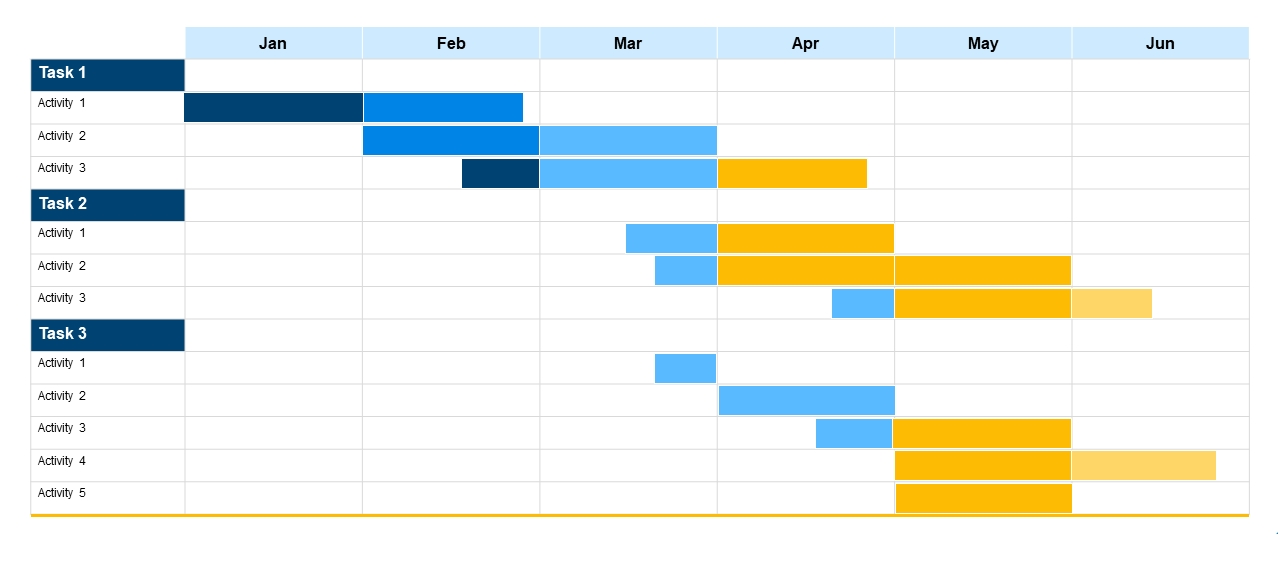
\includegraphics[width=1\textwidth]{./images/gantt.jpg}
    \caption{Diagramme de Gantt}
\end{figure}


%%%%%%%%%%%%%%%%%%%%%%%%%%%%%%%%%%%%%%%%%%%%%%%%%%%
%%% Exemple liste à puces
\section{Exemple de liste à puces}
\paragraph{}
\begin{itemize}[label=$\circ$]
    \item élément 1
    \item élément 2
    \item élément 3
    \item élément 4
    \begin{itemize}
        \item sous-élément 1
        \item sous-élément 2
        \item sous-élément 3
        \item sous-élément 4
    \end{itemize}
\end{itemize}

%%%%%%%%%%%%%%%%%%%%%%%%%%%%%%%%%%%%%%%%%%%%%%%%%%%
%%% Exemple liste numérotée
\section{Exemple de liste numérotée}
\paragraph{}
\begin{enumerate}
    \item élément 1
    \item élément 2
    \item élément 3
    \item élément 4
     \begin{enumerate}
        \item sous-élément 1
        \item sous-élément 2
        \item sous-élément 3
        \item sous-élément 4
    \end{enumerate}
\end{enumerate}

%%%%%%%%%%%%%%%%%%%%%%%%%%%%%%%
%%% Conculsion du chapitre 
\section*{Conclusion}
\addcontentsline{toc}{section}{Conclusion}
\paragraph{}
\lipsum[1]
